\section{Algebraic Moment Closures}
\label{sec:algebraicClosure}

Algebraic moment closures for the two-moment model are computationally efficient as they provide the Eddington factor in Eq.~\eqref{eq:eddingtonTensor} in closed form as a function of the density $\cJ$ and the flux factor $h=|\vect{\cH}|/\cJ$.  
For this reason they are widely used in applications where radiation transport plays an important role --- including simulation of neutrino transport in core-collapse supernovae \cite{roberts_etal_2016} and compact binary mergers \cite{foucart_etal_2015}.  
The family of algebraic closures we consider in this paper can be written in the form \cite{cernohorskyBludman_1994}
\begin{equation}
  \chi(\cJ,h)=\f{1}{3}+\f{2\,(1-\cJ)\,(1-2\cJ)}{3}\,\Theta\Big(\f{h}{1-\cJ}\Big),
  \label{eq:eddingtonFactor}
\end{equation}
where the closure function $\Theta(x)$ varies with the specifics of the closure procedure.  
We will consider two basic closure procedures in more detail below: the maximum entropy (ME) closure and the Kershaw (K) closure.  

\paragraph{Low Occupancy Limit}
We note in passing that in the low occupancy limit ($\cJ\ll1$), the Eddington factor in Eq.~\eqref{eq:eddingtonFactor} becomes independent of $\cJ$; i.e.,
\begin{equation}
  \chi(\cJ,h)\to\chi_{0}(h)=\f{1}{3}+\f{2}{3}\,\Theta\big(h\big).  
  \label{eq:eddingtonFactorLow}
\end{equation}

\subsection{Maximum Entropy (ME) Closure}

For the two-moment model, the ME closure constructs the least biased angular distribution based on the limited information available (i.e., $\cJ$ and $\vect{\cH}$) \cite{cernohorskyBludman_1994}.  
The ME distribution $f_{\mbox{\tiny ME}}(\omega)$ is found by maximizing the entropy functional, which for particles obeying Fermi-Dirac statistics is given by
\begin{equation}
  S[f_{\mbox{\tiny ME}}] 
  = \int_{\bbS^{2}}\big[\,(1-f_{\mbox{\tiny ME}})\log(1-f_{\mbox{\tiny ME}}) + f_{\mbox{\tiny ME}}\log f_{\mbox{\tiny ME}}\,]\,d\omega,
  \label{eq:entropyFunctional}
\end{equation} 
subject to the constraints
\begin{equation}
  \f{1}{4\pi}\int_{\bbS^{2}}f_{\mbox{\tiny ME}}(\omega)\,d\omega=\cJ
  \quad\text{and}\quad
  \f{1}{4\pi}\int_{\bbS^{2}}f_{\mbox{\tiny ME}}(\omega)\,\vect{\ell}(\omega)\,d\omega=\vect{\cH}.  
  \label{eq:closureConstraints}
\end{equation}
From the variation of the entropy functional in Eq.~\eqref{eq:entropyFunctional} with respect to $f_{\mbox{\tiny ME}}$, and introducing Lagrange multipliers to enforce the constraints in Eq.~\eqref{eq:closureConstraints}, the ME distribution takes the general form
\begin{equation}
  f_{\mbox{\tiny ME}}(\omega;a,\vect{b})=\f{1}{e^{a + \vect{b}\cdot\vect{\ell}}+1}, 
  \label{eq:fME}
\end{equation}
which can be further simplified by a change of coordinates $a + \vect{b}\cdot\vect{\ell}=a + b\,\mu$, where $b=|\vect{b}|$, and $\mu\in[-1,1]$ is the cosine of the angle between $\vect{b}$ and $\vect{\ell}$.  
The Lagrange multipliers are implicit functions of $\cJ$ and $|\vect{\cH}|$.  
The ME distribution function satisfies $0 \le f_{\mbox{\tiny ME}} \le 1$, but $a$ and $b$ are unconstrained.  

Chernohorsky \& Bludman \cite{cernohorskyBludman_1994} postulate (but see \cite{lareckiBanach_2011}) that, as a function of the so-called flux saturation $x=h/(1-\cJ)$, the closure function $\Theta(x)$ is independent of $\cJ$ and can be written explicitly in terms of the inverse Langevin function.  
They also provide a polynomial fit (accurate to $2\%$) given by
\begin{equation}
  \Theta_{\mbox{\tiny ME}}^{\mbox{\tiny CB}}(x)
  =\f{1}{5}\,\big(\,3-x+3\,x^{2}\,\big)\,x^{2}.
  \label{eq:closureMECB}
\end{equation}
More recently, Larecki \& Banach \cite{lareckiBanach_2011} have shown that the explicit expression given in \cite{cernohorskyBludman_1994} is not exact, and provide another approximate expression
\begin{equation}
  \Theta_{\mbox{\tiny ME}}^{\mbox{\tiny BL}}(x)
  =\f{1}{8}\,\big(\,9\,x^{2}-5+\sqrt{33\,x^{4}-42\,x^{2}+25}\,\big),
  \label{eq:closureMEBL}
\end{equation}
which is accurate to within $0.35\%$.  
On the interval $x\in[0,1]$, the curves given by Eqs.~\eqref{eq:closureMECB} and \eqref{eq:closureMEBL} lie practically on top of each other.  

\subsection{Kershaw (K) Closure}

The basic principle behind Kershaw closure is derived from the fact that the realizable set defined by $(\cJ, \vect{\cH}, \vect{K})$ is convex.
Due to the convexity, any element in the convex set be expressed as a convex combination of two elements that on the set boundary, and vice versa.
That is,
\begin{align}
 \chi(\cJ,h) = \beta  \chi_{L}(\cJ,h) + (1-\beta) \chi_{U}(\cJ,h),
\end{align}
with $\chi_{L}$ and $\chi_{U}$ be the boundary elements, and $\beta \in [0,1]$. 
The Kershaw closure uses a convex combination that determined by the isotropic distribution case to approximate $\chi(\cJ,h)$:
\begin{align}
 \chi(\cJ,0)  &= \dfrac{1}{3},\\
\chi_{L}(\cJ,h) & = \dfrac{1}{3}\cJ^2 + h^2, \\
\chi_{U}(\cJ,h) & = \left( 1 - \cJ + \dfrac{1}{3}\cJ^2 \right) - \dfrac{h^2 \cJ}{1-\cJ},
\end{align}
$\chi_{L}$ and $\chi_{U}$ are given by the Heaviside function with Fermi-Dirac statistic function, and
\begin{align}
\beta = \dfrac{2 - \cJ}{3}.
\end{align}
Then the Kershaw closure function $\Theta(x)$ reads (Banach \& Larecki \cite{banachLarecki_2017a}):
\begin{equation}
  \Theta_{\mbox{\tiny K}}^{\mbox{\tiny BL}}(x)=x^{2}
\end{equation}

Figure~\ref{fig:MabWithDifferentClosure} illustrates the behavior of these four closure.
As it shows, Minerbo closure (right bottom) is the only one among those four closures that does not preserve realizability.
\begin{figure}[h]
  \centering
  \begin{tabular}{cc}
    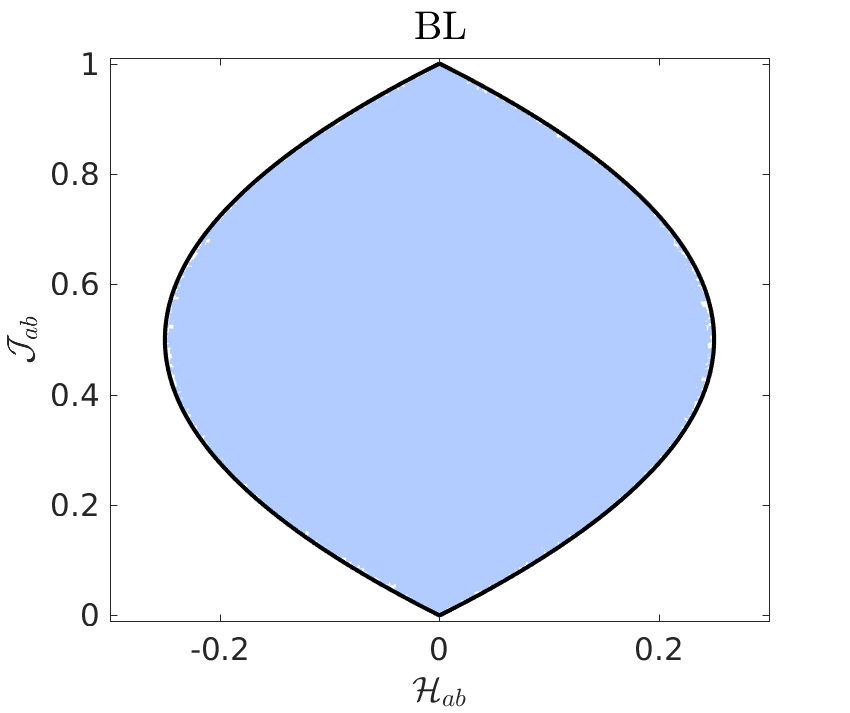
\includegraphics[width=0.5\textwidth]{figures/MabWithBLME}
    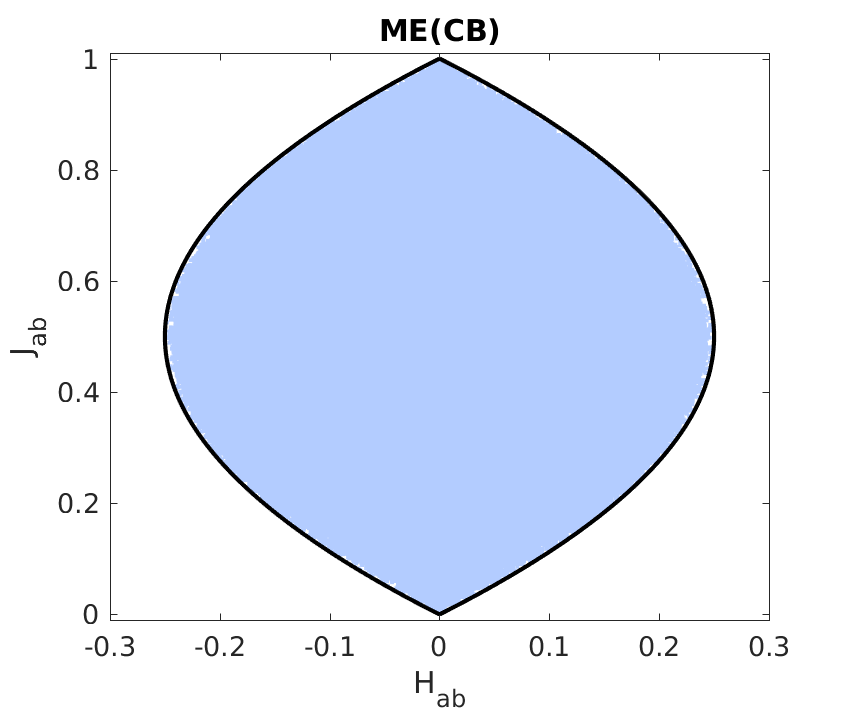
\includegraphics[width=0.5\textwidth]{figures/MabWithCBME} \\
    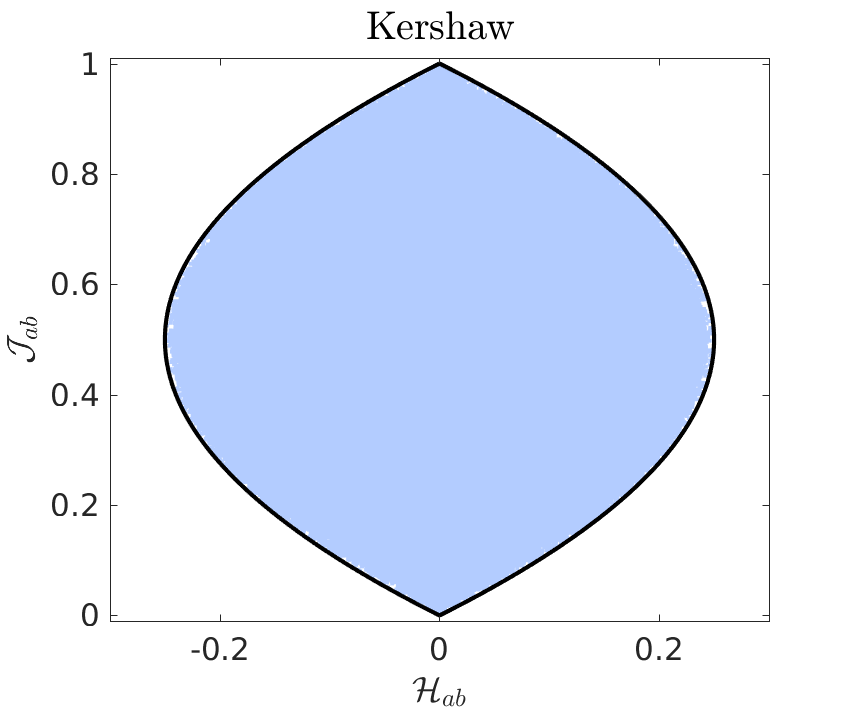
\includegraphics[width=0.5\textwidth]{figures/MabWithBLKS}
    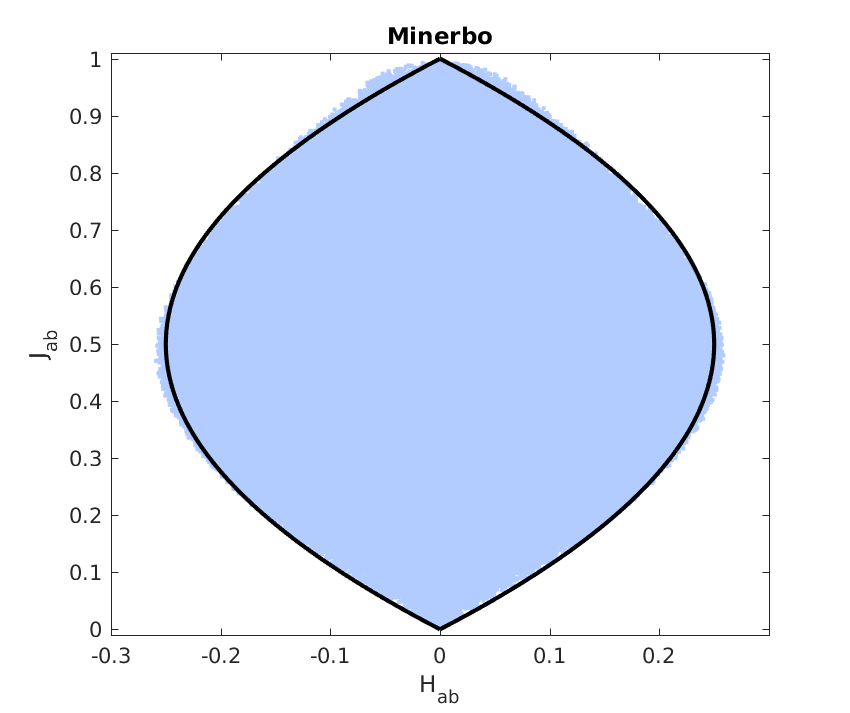
\includegraphics[width=0.5\textwidth]{figures/MabWithMI}
  \end{tabular}
   \caption{Illustration of $\vect{\cM}_{ab}$ with four different closures: Banach \& Larecki maximum entropy closure (left top), Chernohorsky \& Bludman maximum entropy closure (right top), Kershaw closure (left bottom), and Minerbo closure (right bottom).
   Total $10^{6}$ pairs of random Fermi-Dirac distribution were generated.
   With these pairs, $\vect{\cM}_{ab}$ with different closures were calculated separately and marked with light-blue points.
   Black lines define the boundary of $\cR$: $\gamma(\vect{\cM}) = 0$.}
  \label{fig:MabWithDifferentClosure}
\end{figure}